\section{Introdcucción}

Este documento explica los avances realizados de la semana octava a  la décima el cual corresponde al periodo 22 de septiembre $-$ 12 de octubre( ver Figura \ref{fig:cronograma}) del año 2019. las actividades reportadas son:

\begin{enumerate}
	\item Incremento del corpus
	\item Selección de noticias aptas para el proceso de entrenamiento	
	\item Entrenamiento de algoritmos
	\item Validación cruzada
	\item Diseño de la página web
\end{enumerate} 

\begin{figure}[h]
\centering
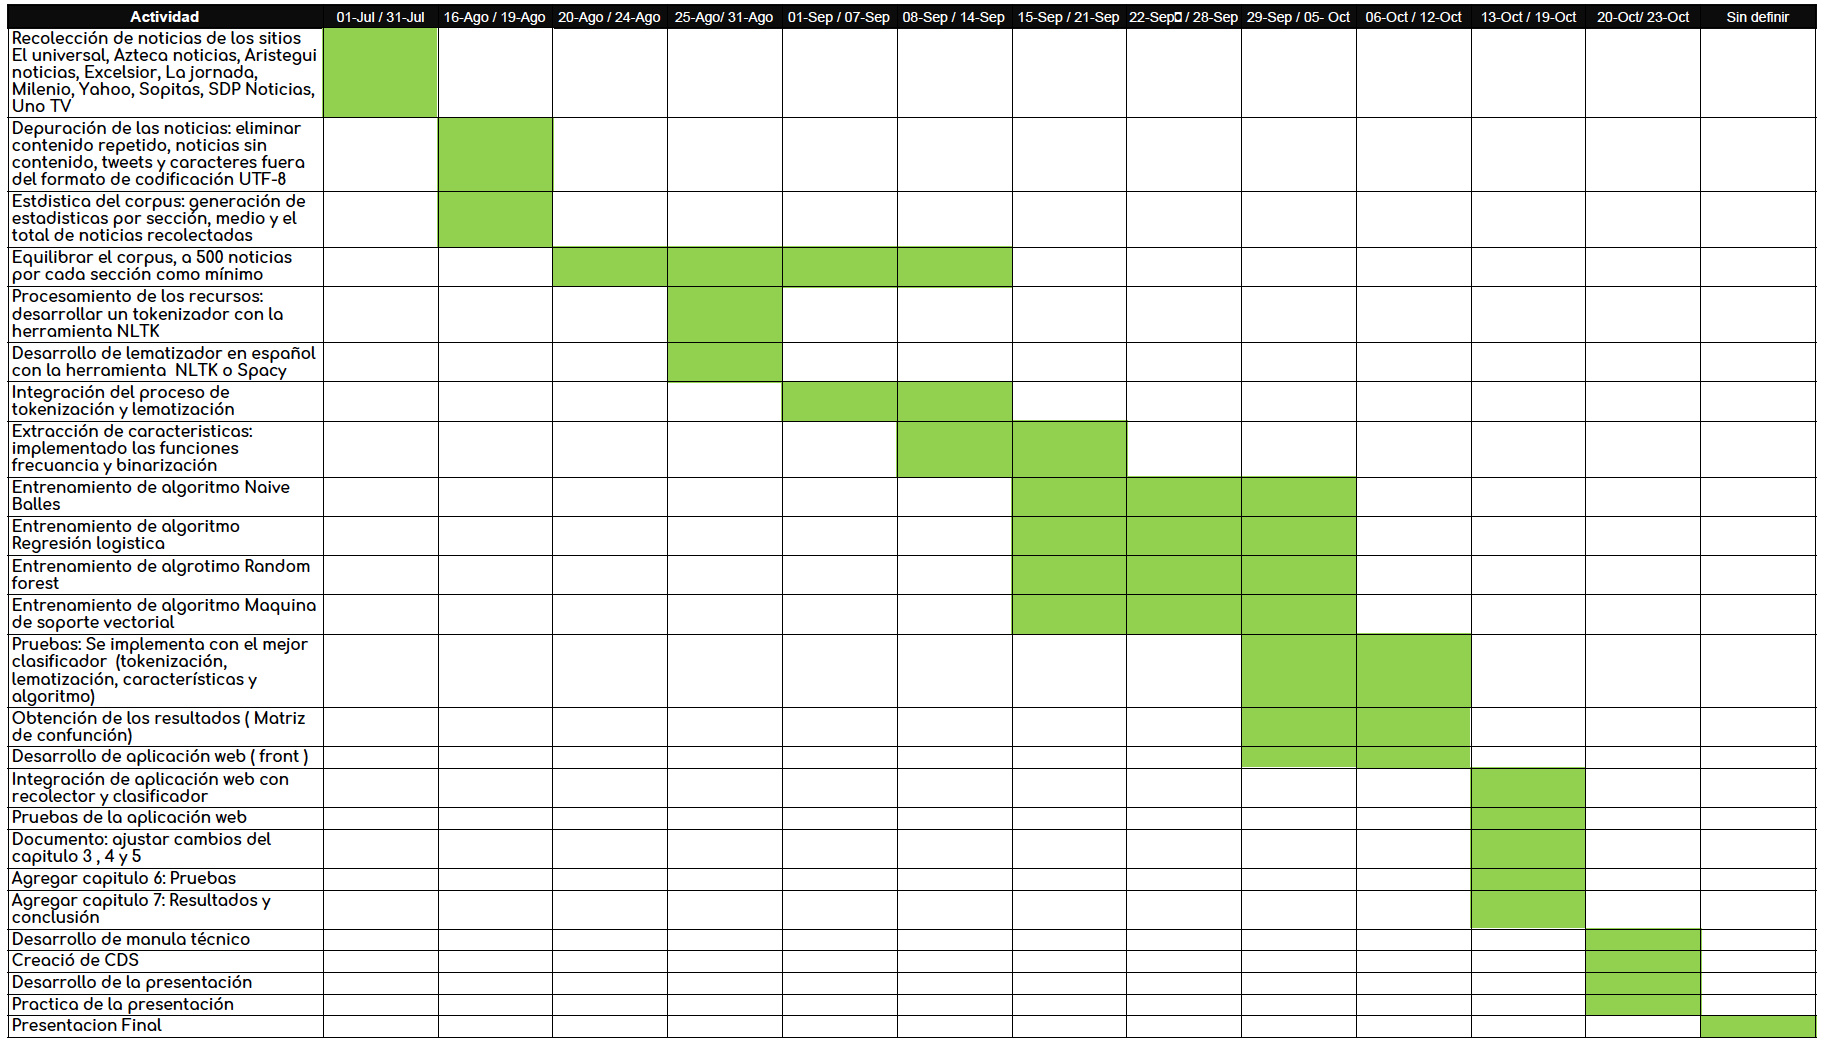
\includegraphics[scale=0.4]{imagenes/Cronograma.png}
\caption{Cronograma correspondiente al trabajo terminal 2}
\label{fig:cronograma}
\end{figure}

%--------------------------------------------------------------------------------------------------%
\section{Incremento del corpus}

Como meta del número de noticias para formar el corpus se propuso 500 noticias como mínimo por cada sección ( las cuales son \textbf{ciencia y tecnología}, \textbf{deportes}, \textbf{política}, \textbf{cultura} y \textbf{economía}) sin embargo con vías de alcanzar mejores resultados en el entrenamiento de los algoritmos, se incrementó el número de artículos a 700, es decir 3500 noticias en total.\\

Para este procedimiento se recolectaban noticias cada 3 días de los sitios web:

\begin{itemize}
	  \item \textbf{El Universal}: https://www.eluniversal.com.mx/
      \item \textbf{La Jornada}: https://www.jornada.com.mx/
	  \item \textbf{Aristegui Noticias}: https://aristeguinoticias.com/
	  \item \textbf{Sopitas}: https://www.sopitas.com/
      \item \textbf{TV Azteca}: https://www.aztecanoticias.com.mx/
      \item \textbf{Televisa}: https://noticieros.televisa.com/
      \item \textbf{Once Noticias}: https://www.oncenoticias.tv/
      \item \textbf{El economista}: https://www.eleconomista.com.mx/
\end{itemize}

Se implementaron las arañas (\textit{crawler}) desarrolladas en el trabajo terminal 1. Además se especializaron algunos algoritmos para obtener mas noticias de la sección \textbf{cultura.}\\

El resultado de las noticias recolectadas se muestra en la Figura \ref{fig:recoleccion}:

\begin{figure}[h]
\centering
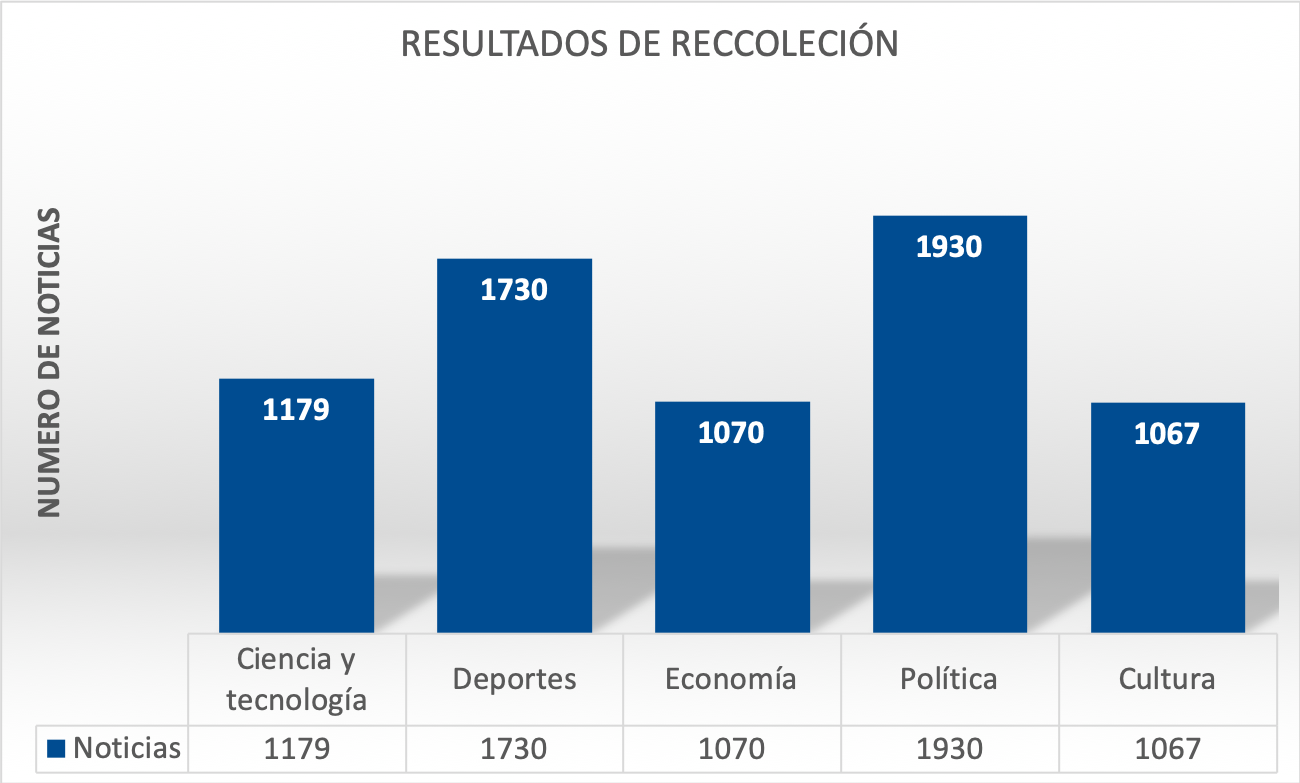
\includegraphics[scale=0.4]{imagenes/Resultados/Recoleccion.png}
\caption{Gráfica de recolección de noticias}
\label{fig:recoleccion}
\end{figure}

%--------------------------------------------------------------------------------------------------%
\section{Selección de noticias aptas para el proceso de entrenamiento}

Una vez obtenidas las noticias se limpiaron y se seleccionaron los artículos aptos para ser usadas en el proceso de entrenamiento, mediante la aplicación de un filtro, el cual verifica que un texto contenga como mínimo 180 palabras. La meta consistió en obtener 700 noticias validas por sección, sin embargo hay secciones que obtuvieron mas de dicho número  y otras un poco menos. Cabe destacar que las secciones se  acotaron a 700 noticias, los resultados obtenidos se muestra en la figura \ref{fig:filtro}. 


\begin{figure}[h]
\centering
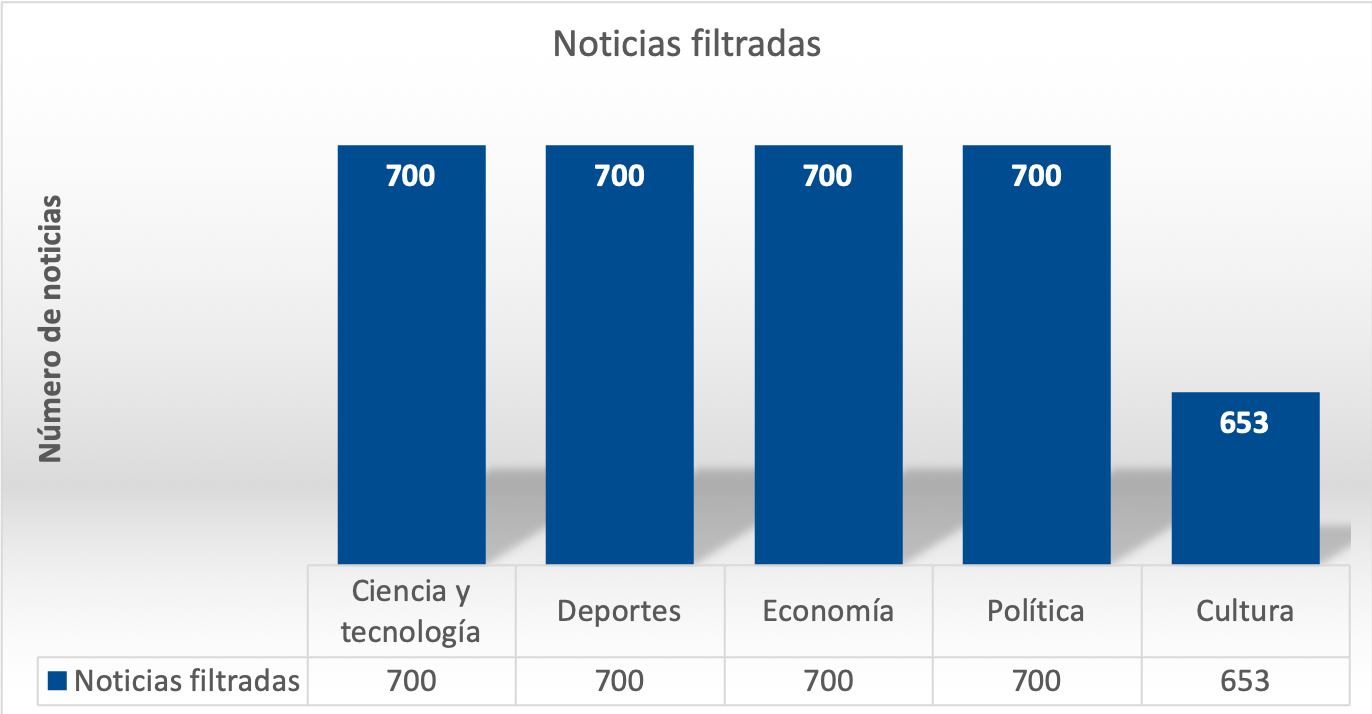
\includegraphics[scale=0.4]{imagenes/Resultados/Filtrado.png}
\caption{Gráfica de noticias obtenidas con mas de 180 palabras}
\label{fig:filtro}
\end{figure}

%--------------------------------------------------------------------------------------------------%
\section{Entrenamiento de algoritmos}

Se entrenaron los algoritmos propuestos en trabajo terminal 1 los cuales son: \textbf{Naive bayes}, \textbf{Random forest}, \textbf{Maquina de soporte vectorial} y \textbf{Regresión logística}.\\

%\begin{itemize}
%	\item \textbf{Naive bayes}
%	\item \textbf{Random forest}
%	\item \textbf{Maquina de soporte vectorial}
%	\item \textbf{Regresión logística}
%\end{itemize}

El proceso de entrenamiento se muestra en la Figura \ref{fig:clasificacion}

\begin{figure}[h]
\centering
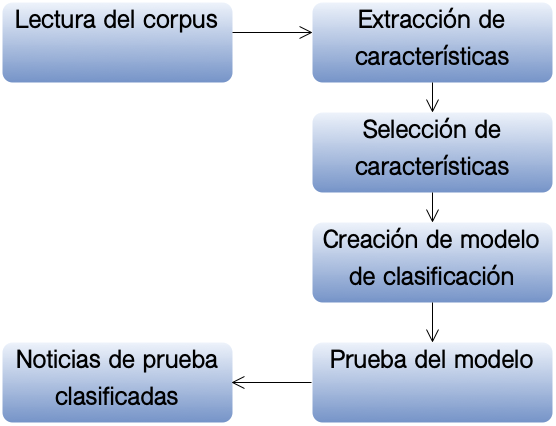
\includegraphics[scale=0.35]{imagenes/Resultados/Clasificacion.png}
\caption{Proceso de entrenamiento}
\label{fig:clasificacion}
\end{figure}

\begin{enumerate}

	\item \textbf{Lectura del corpus}:Consiste en leer las noticias almacenadas en un archivo tipo CSV, con la librería \textbf{Pandas} de \textbf{python}. Se obtiene el título y la redacción del artículo.

	\item \textbf{Selección de características}: Se identifican las palabras que son comunes para cada sección por ejemplo, fútbol, jugador y gol son palabras que aparecen en el tópico de deportes. 

	\item \textbf{Extracción de características}: Se crea un espacio vectorial por cada noticia donde cada elemento del vector representa la presencia o ausencia de una característica(palabra). Cabe mencionar que las características son extraídas de 2 formas, binario(donde 1 representa la presencia de la característica y 0 la ausencia) y por frecuencia ( donde se cuenta la cantidad de veces que cada característica aparece). Se ha implementado \textbf{CountVectorizer} de la librería \textit{scikit learn} para este proceso.

	\item \textbf{Creación del modelo}: Los modelos creados son entrenados de forma supervisada, se brinda un conjunto de noticias (es decir el espacio vectorial de cada artículo) y el resultado de la clasificación para crear el modelo. Se ha implementado los algoritmos de la librería \textbf{sckit learn}.

	\item \textbf{Prueba del modelo}: EL corpus se divide en 2 partes, donde la primera es llamada \textbf{conjunto de entrenamiento} (el cual consiste en el 93\% las noticias) y la segunda es llamada \textbf{conjunto de prueba} (el cual consiste en 7\% del corpus).

	\item \textbf{Noticias de prueba clasificadas}: Se obtiene un vector numérico de resultados el cual muestra la clasificación de las noticias de prueba. donde \textbf{0}:Deportes, \textbf{1}:Economía, \textbf{2}:Política, \textbf{3}:Cultura y \textbf{4}:Ciencia y tecnología.
	
%	\begin{itemize}
%		\item \textbf{0}:Deportes
%		\item \textbf{1}:Economía
%		\item \textbf{2}:Política
%		\item \textbf{3}:Cultura
%		\item \textbf{4}:Ciencia y tecnología
%	\end{itemize}

\end{enumerate}


%--------------------------------------------------------------------------------------------------%

\section{Validación cruzada}

Para medir la eficiencia de cada algoritmo se genera un conjunto de noticias de entrenamiento y otro de prueba sin embargo, la selección de estas noticias puede ser manipulados para obtener mejores resultados. Para evitar esta situación se generan las pruebas con un método llamado validación cruzada el cual consiste en partir el corpus en pliegues y generar las pruebas mas de una vez (ver Figura \ref{fig:validacioncruzada} ) y calcular la eficiencia promedio del clasificador, de esta forma se obtienen resultados mas robustos y confiables.


\begin{figure}[h]
\centering
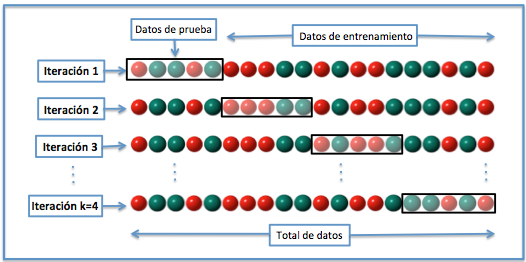
\includegraphics[scale=0.5]{imagenes/Resultados/validacioncruzada.png}
\caption{Validación cruzada}
\label{fig:validacioncruzada}
\end{figure}


\subsection[Métricas]{Métricas de evaluación}

Para medir la eficiencia del clasificador se hace uso de la matriz de confusión.\\

\textbf{Matriz de confusión}\\

Una matriz de confusión es una representación de la información de los resultados obtenidos por un
clasificador, dicha matriz suele ser de tamaño n x n, donde n es es el número de clases diferentes con
las que se están trabajando.

\begin{figure}[h]
	\centering
	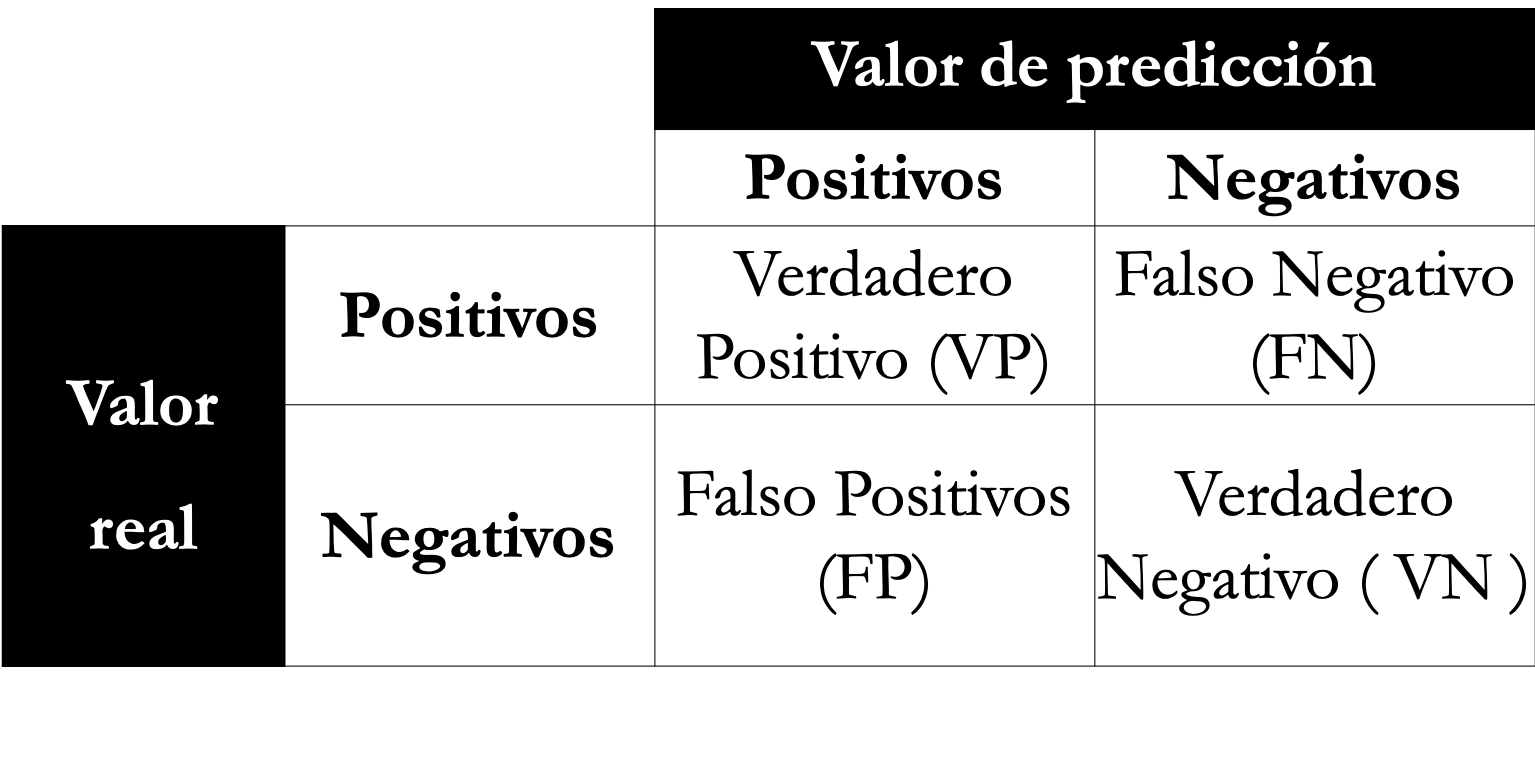
\includegraphics[scale=.35]{imagenes/Resultados/MatrizC.png}
	\caption{Matriz de confusión}
	\label{Fig:mconfu}
\end{figure}

La Figura \ref{Fig:mconfu} muestra un ejemplo de matriz de confusión con dos clases, la cual ejemplifica de
manera adecuada las diferentes entradas de la misma, entra las que se encuentran:


Gracias a la matriz de confusión, es posible obtener ciertas métricas que nos ayudan a evaluar el modelo
de aprendizaje. Entre las que se encuentran:\\


\textbf{Exactitud}: es la proporción del número total de predicciones que son correctas respecto al total.
Se determina utilizando la ecuación:

\begin{equation}\label{eq:1}
	Exactitud = \frac{VP+VN}{VP+VN+FN+FP}
\end{equation}

\textbf{Recall}: Es la proporción de predicciones positivas que fueron correctamente clasificadas. Se determina
utilizando la ecuación:


\begin{equation}\label{eq:2}
	Recall = \frac{VP}{VP+FP}
\end{equation}


\textbf{Precisión}: Es la proporción de predicciones positivas que se clasificaron correctamente. Se determina
con la siguiente ecuación:


\begin{equation}\label{eq:3}
	Precision = \frac{VP}{VP+FN}
\end{equation}


\textbf{F-Measure (F1)}: Se interpreta como la media armónica entre Precisión y Recall. Se determina
con la siguiente ecuación:

\begin{equation}\label{eq:3}
	 F-Measure = 2 \cdot \frac{precision \cdot recall}{precision+recall}
\end{equation}





Para estas prueba pruebas se han generado 3 pliegues en la validación cruzada, la Figura \ref{fig:matrizfrecuencia} muestra los resultados obtenidos al extraer las características por frecuencia y la Figura \ref{fig:matrizbinario} muestra los resultado obtenidos al extraer las características de forma binaria.

\begin{figure}[h]
\centering
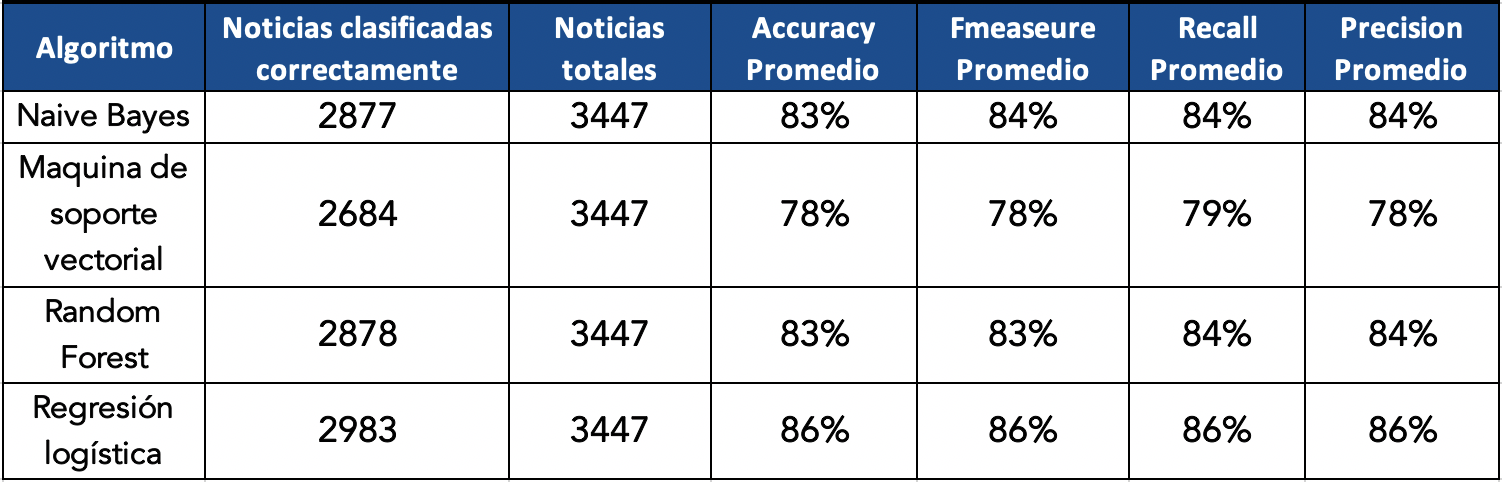
\includegraphics[scale=0.45]{imagenes/Resultados/MatrizFrecuencia.png}
\caption{Resultados de entrenamiento modo Frecuencia}
\label{fig:matrizfrecuencia}
\end{figure}

\begin{figure}[h]
\centering
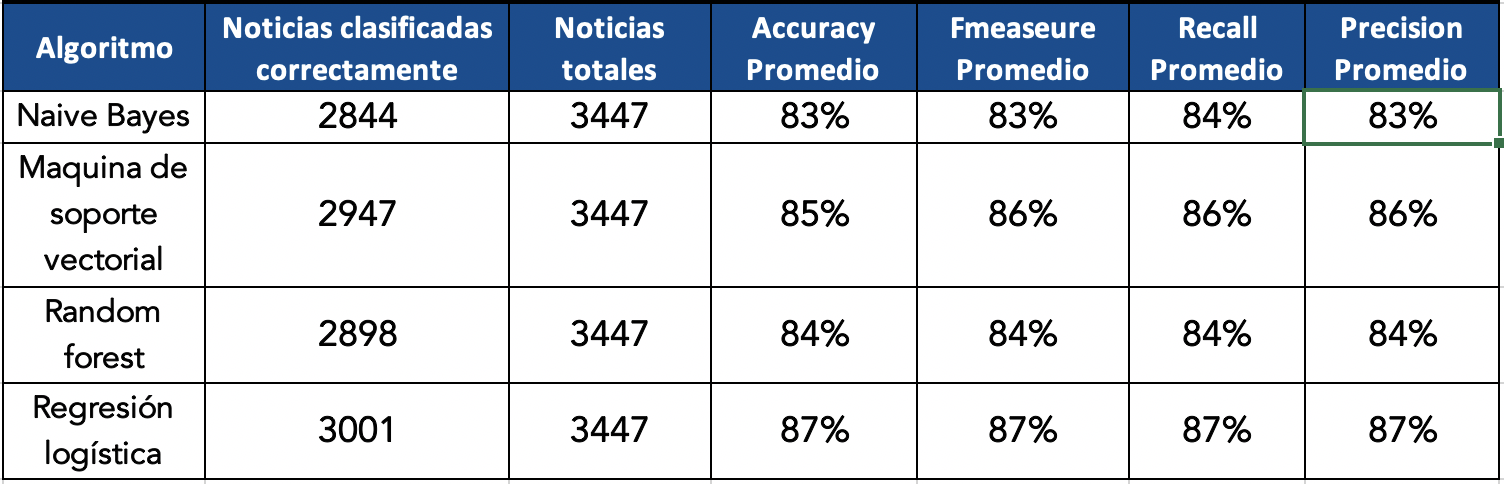
\includegraphics[scale=0.45]{imagenes/Resultados/MatrizBinario.png}
\caption{Resultados de entrenamiento en modo binario}
\label{fig:matrizbinario}
\end{figure}


Se puede observar que el mejor resultado es dado por el clasificador \textbf{Regresión logística}, al extraer las características de forma bianaria con un \textit{Accuracy, Fmeasure, Recall y Precision} de un 87\%. Cabe mencionar que esta no son las pruebas finales de los clasificadores el siguiente paso es variar los parámetros usados en cada clasificador para obtener el mejor clasificador con los mejores parámetros.